\renewcommand\evenpagerightmark{{\scshape\small Scale-up}}
\chapter[Scale-up]%
{Scale-up}
\label{Scale-up}

\section{The geometry}
\subsection{What is required}

The main objective of this burner is to investigate the effect of swirl on diffusion flame in an oxycombustion with a coaxial shape. The  work on ATR30 burner has been to establish an environment similar to the Freiberg OPTISOS study (in terms of flame topology ) with scale-up rules : conservation of geometry, speeds, swirl, $Z_{st}$, $J$. The aim of this burner is to be studied in a very similar environment as the study on ATR30 burner. Consequently, though the geometry is to evolve, a particular care is paid so that the speeds and the mass flows remain constant.

Let us make a bill of specifications for that burner :
\begin{enumerate}
\item The Swirl number must be modular from 0 to 2 (margins included)
\item The outlet speeds must be the same as the OPTYSOS study
\item The mass flows have to be similar to the Calhory sizing study with ATR30 burner
\item The internal axial swirled pipe will be the same as the ATR30 burner (since it is already crafted)
\item The $H_{2}O$ intermediate injection will not be used
\item The geometry must be convenient with combustion (in particular, the wall between the fuel and the oxidant must not exceed $1-2mm$, so as to prevent the flame from fixing itself in the shear stress boundary limit)  
\item The shape must be as simple as possible
\end{enumerate}
One must acknowledge that these objectives do not seem so ambitious, but the following study stresses the difficulties.

\begin{figure}[h!]
  \centering
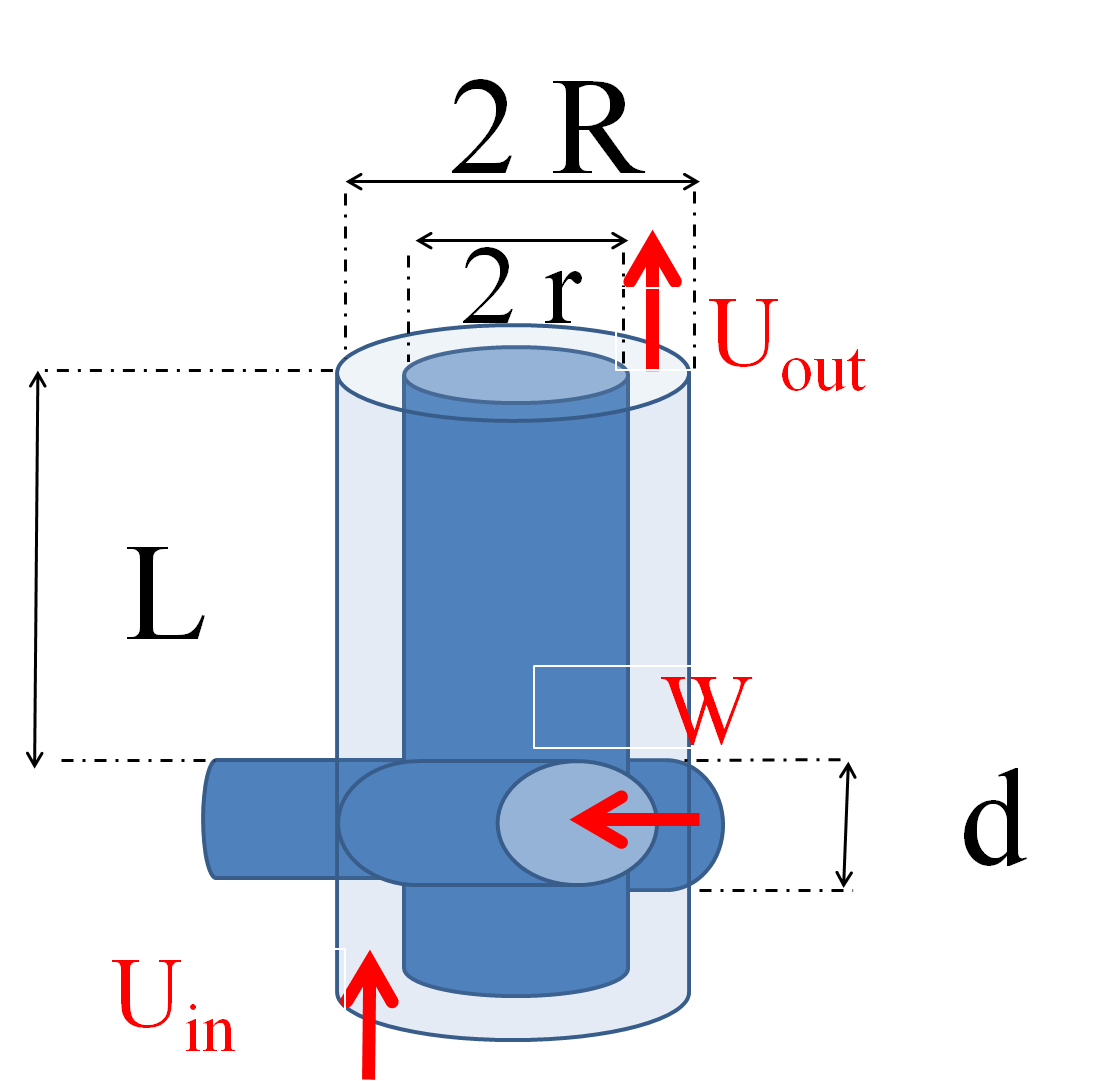
\includegraphics[width=0.50\textwidth]{fig/Proto.png}
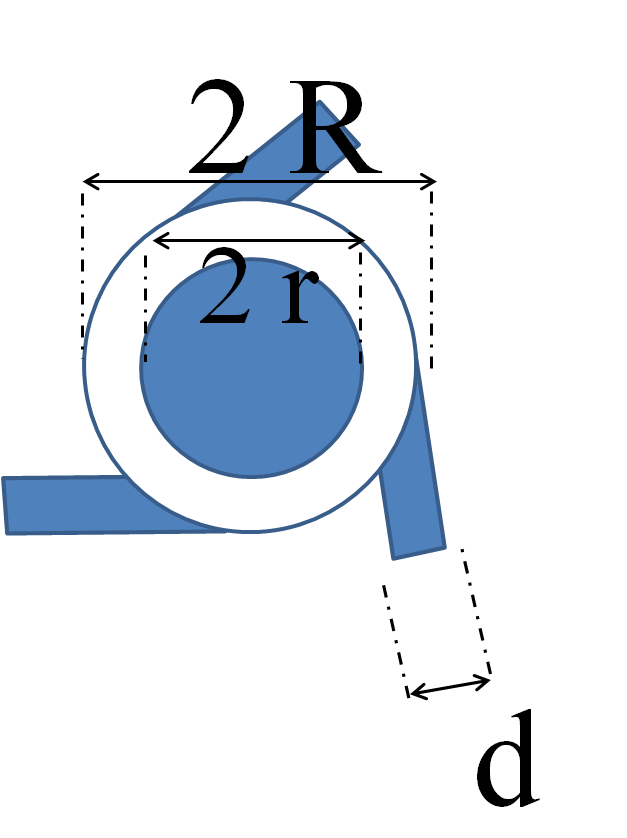
\includegraphics[width=0.40\textwidth]{fig/proto_dessus.png}
  \caption{Notations and hypothetical geometry of the prototype burner}
 \label{proto_pipe}
\end{figure}
Figure \ref{proto_pipe} gives the geometrical notations. Only the outer flow is studied, since the internal pipe is the pipe of the ATR30norm, whose geometry and swirl are already given.

Let us call $U_{out}$ the speed at the outlet of the outer pipe (at the top of the figure), $U_{in}$ the speed at the inlet of the outer pipe and $W$ the speed in the tangential pipes.

The mass conservation gives :
\begin{equation}
\dot{m_{in}}+\dot{m_{tangential}}=\dot{m_{out}}
\end{equation}


The fluid being the same in the axial and the tangential injections, we have :
\begin{equation}
U_{in}+W \frac{A_{\theta}}{A_{z}}=U_{out}
\end{equation}


\subsection{The problem of tangential speed}

In this section, it is demonstrated that the geometrical area providing the tangential injections needs to be as big as possible.

Let us consider the case where the swirl is maximum, so that the mass flow entirely comes from the tangential injections, and the injected axial flow is null. Then the mass conservation gives :
\begin{equation}
W=U_{out} \frac{A_{z}}{A_{\theta}}
\end{equation}


For practical reasons, $W$ is required smaller than $75m/s$. $U_{out}$ is the speed we want to fit to Optysos study, so it is fixed to $U_{out}=75m/s$. 

\subsection{First try with circular pipes injections}

It is demonstrated that the pipe geometry for the tangential injections seems not a good solution.

If the axial pipe goes from $r$ to $R$, there is only the room $d=R-r$ to put a circular pipe of diameter $d$ between the boundaries of the axial pipe.
If we compute the ratio :
\begin{equation}
\frac{A_{\theta}}{A_{z}}=\frac{N\pi d^2/4}{\pi (R^2-r^2)}
\end{equation} N being the number of tangential injections

Then, we  have :
\begin{equation}
 \frac{A_{\theta}}{A_{z}}=\frac{N(R-r)}{4 (R+r)}
\end{equation}

 since $r$ is fixed to $7.05mm$, we see that we need $R$ big and $N>4$  so that $W<75m/s$.
 
 This is impossible to achieve. The first conclusion is that using circular pipes for tangential injections as it is the case in fig \ref{proto_pipe} will give too big tangential speeds.
 
 \subsection{Paralepipedic injections }

Let us now consider that there are $N$ injections of paralepipedic pipes, of diameter $d$ and height $H$, as it is shown in fig \ref{proto_par}

\begin{figure}[h!]
  \centering
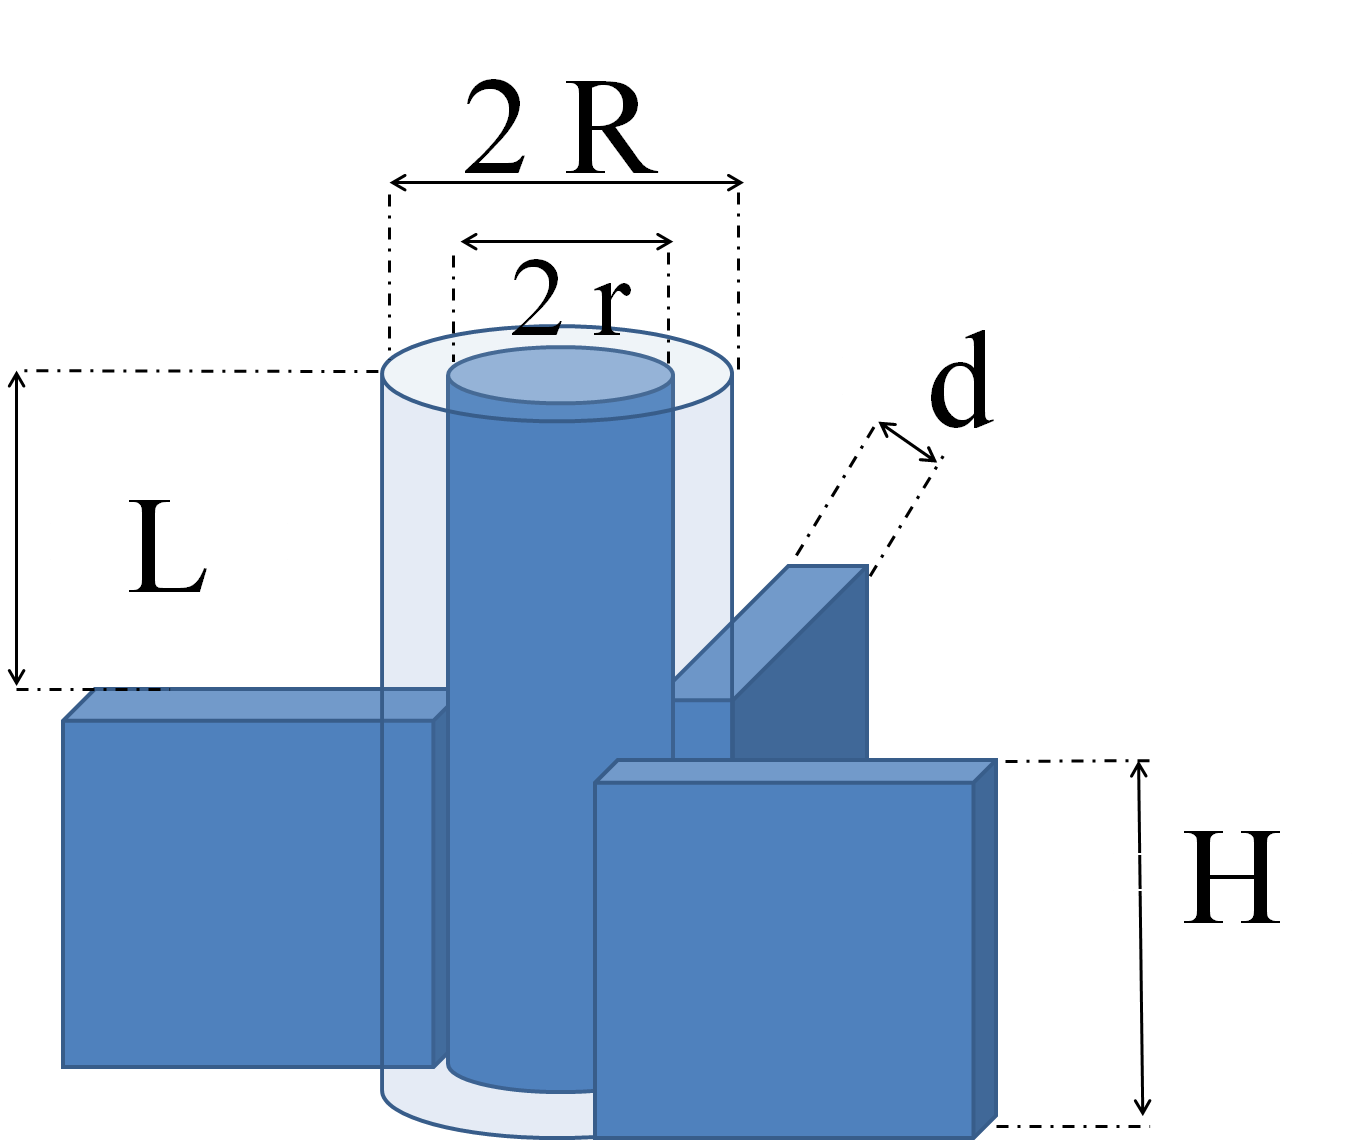
\includegraphics[width=0.45\textwidth]{fig/proto_par.png}
  \caption{Notations and hypothetical geometry of the prototype burner}
 \label{proto_par}
\end{figure}
It has been seen that $d$ must be maximized : $d=R-r$. The parameter H has now to be sized with :
\begin{equation}
W =U_{out}\frac{A_{z}}{A_{\theta}}
\end{equation}


Hence, it goes :
\begin{equation}
W=U_{out}\frac{\pi (R^2-r^2)}{NdH}
\end{equation}

Multiple tangential injections being complicated to craft, it is considered that the maximum injection number is $N=3$. In order to limit the tangential speed to 75m/s in the "worst case" (the flow is entirely tangential), we have : $H=\frac{\pi (R^2-r^2)}{Nd}=20mm$ .

Though a paralepiped injection may be harder to craft, for now it is the only investigated solution to prevent from high speeds in the burner.

\subsection{The computation of the swirl number}

The difficulties of the computation of the swirl number have previously been underlined : every mistakes or discussions starts from the assumptions on the tangential $W$ profile (constant, solid body rotation, vortex...). 

As it as been seen, in case of a swirled annular pipe, the profile $W(r)=cste \cdot \delta(r)_{r \in [R-d,R]}$ has been chosen, as it is shown in fig \ref{proto_profile}.

\begin{figure}[h!]
  \centering
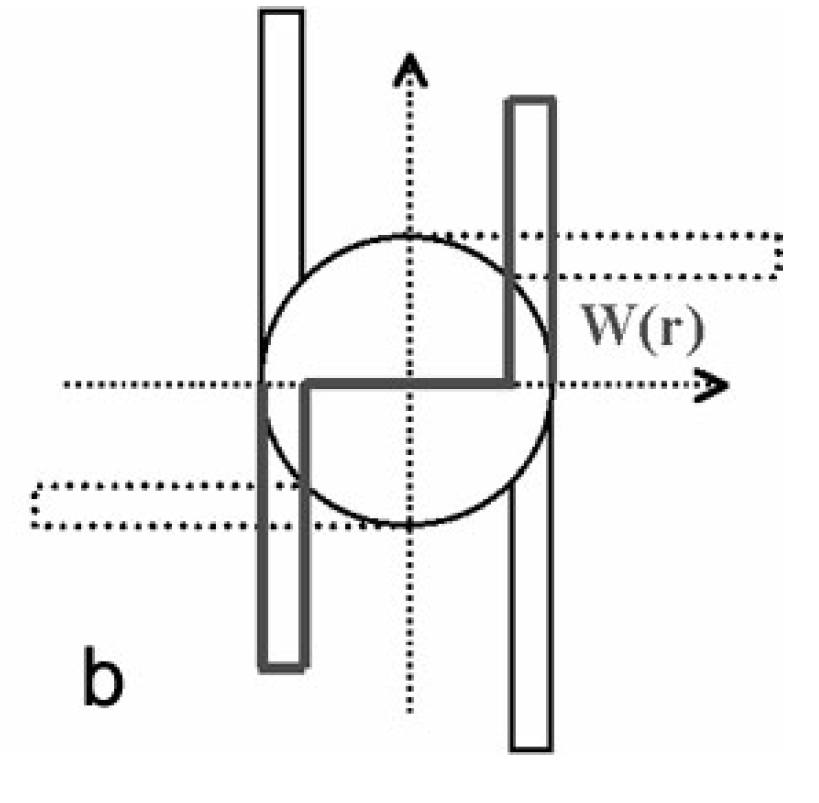
\includegraphics[width=0.45\textwidth]{fig/proto_W_profile.PNG}
  \caption{Notations on W(r) profile}
 \label{proto_profile}
\end{figure}
We thus have :
\begin{itemize}
\item from $0$ to $r$ : it is the inner pipe with axial swirl, so the speed of the outer annular pipe has no value in that area
\item from $r$ to $R-d$, we have $U_{out}=cste$ and $W(r)=0$
\item from $R-d$ to $R$, we have $U_{out}=cste$ and $W(r)=cste$
\end{itemize}



Here goes the calculations on swirl number:
\begin{equation}
S=\frac{\int_{r}^{R} W \cdot U_{out} r^2 dr}{R\int_{r}^{R}  U_{out}^2 r dr}
\end{equation}

\begin{equation}
S=\frac{W\int_{R-d}^{R} r^2dr}{R U_{out} \int_{r}^{R}  r dr}
\end{equation}

\begin{equation}\label{eq:S_proto_speed}
S=\frac{W \cdot d (R^2+d^2/3-dR)}{U_{out}R(R^2-r^2)/2}
\end{equation}
The mass conservation giving $U_{in}+W \frac{A_{\theta}}{A_{z}}=U_{out}$ , it goes in the general case (with no constraint on the shape of the tangential injection):
\begin{equation}
S=\frac{1}{1+\frac{\dot{m_{in}}}{\dot{m_{\theta}}}}\frac{A_{z}}{A_{\theta}}\frac{2d}{R}\frac{(1+\frac{d^2}{3R^2}-\frac{d}{R})}{1-(\frac{r}{R})^2}
\end{equation}


In case of a rectangular injection, here are the simplifications :
\begin{equation}
S=\frac{1}{1+\frac{\dot{m_{in}}}{\dot{m_{\theta}}}}\frac{2 \pi R}{NH}(1+\frac{d^2}{3R^2}-\frac{d}{R})
\end{equation}


To limit the speed of $W$, $A_{\theta}$ has been maximized as far as $d=R-r$.

Hence, we finally have :
\begin{equation}
S=\frac{1}{1+\frac{\dot{m_{in}}}{\dot{m_{\theta}}}}\frac{2 \pi R}{3NH}(1+\frac{r}{R}(1+\frac{r}{R}))
\end{equation}


Unfortunately, the calculation of this swirl number gives $S=0.81$, which is considered as too small : indeed, that swirl rotation can be dissipated, and let us keep in mind that this swirl is just an approximation of the real Swirl number. Many references record that the LDV-measured swirl number is two times smaller of the computed one. As a conclusion, since the internship wants to investigate large swirl number values, another design is to be found so as to reach higher predicted swirl number.

We can use the results from \ref{eq:S_proto_speed}, where the speed ratio appears :
\begin{equation}
S=\frac{W \cdot d (R^2+d^2/3-dR)}{U_{out}R(R^2-r^2)/2}
\end{equation}


To simplify it with $d=R-r$:
\begin{equation}
S=\frac{W}{U_{out}}\frac{2}{3}\frac{(1+(\frac{r}{R})^2+\frac{r}{R})}{1+\frac{r}{R}}
\end{equation}


$r$ being fixed, $R$ is plotted in figure \ref{proto_plot}. It seems there is no solution with this configuration. The need to take $\frac{W}{U_{out}}$ smaller than 1 makes the swirl very small in every configuration.


\begin{figure}[h!]
  \centering
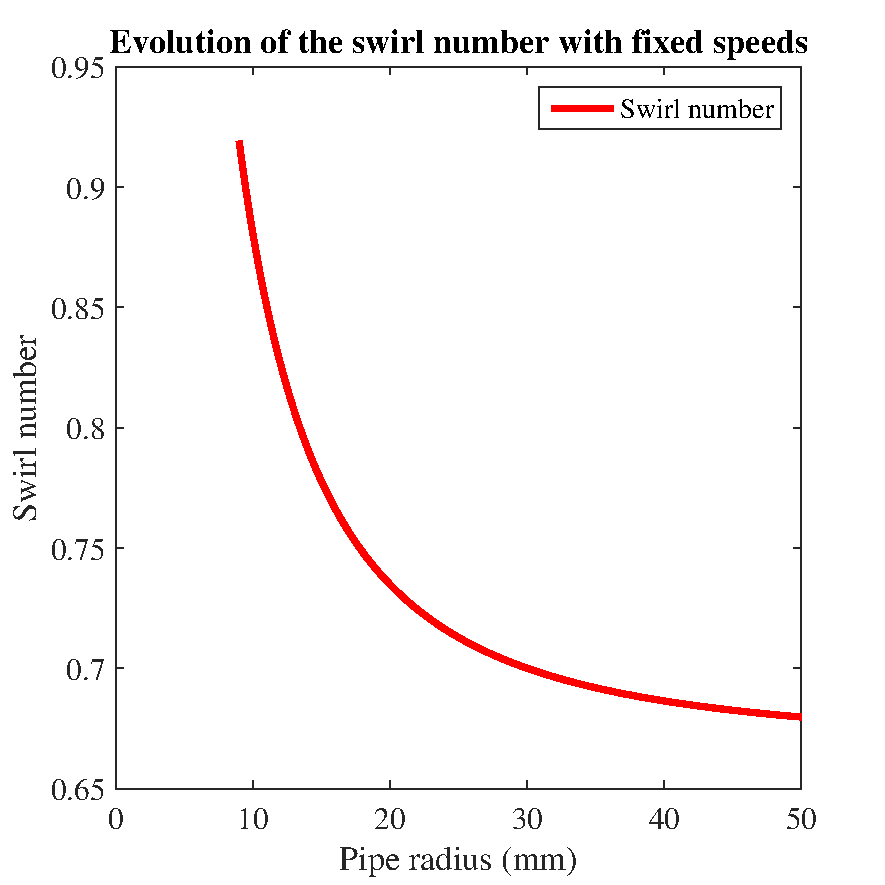
\includegraphics[width=0.7\textwidth]{fig/Proto_burner_Swirl.pdf}
  \caption{Notations on W(r) profile}
 \label{proto_plot}
\end{figure}



